\section{Introduction}\label{introduction}

\begin{frame}{Introduction - Resource Allocation in Open Systems}

The prevalence of open systems -- e.g.~smart grids, cellular networks
and cloud computing -- is driving a demand for `better' solutions to a
standard \textbf{resource allocation problem}:

\begin{itemize}
\tightlist
\item
  How to collectivise and distribute a set of common-pool resources,
  considering

  \begin{itemize}
  \tightlist
  \item
    Fairness
  \item
    Inclusivity
  \item
    Sustainability
  \end{itemize}
\item
  How to overcome problems such as

  \begin{itemize}
  \tightlist
  \item
    No centralised authority
  \item
    No full disclosure
  \item
    Economy of scarcity
  \end{itemize}
\end{itemize}

\end{frame}

\begin{frame}{Computational Justice}

\begin{itemize}
\tightlist
\item
  How resources can be distributed in a \alert{fair} manner?

  \begin{itemize}
  \tightlist
  \item
    How to \textbf{prioritise} requests?
  \item
    What \textbf{fairness criteria} should be considered when judging
    merit (equality, equity, proportionallity, \ldots{})
  \item
    How to \textbf{avoid abuses} in the system (\emph{free-riding},
    deceiving, non-compliancy)
  \end{itemize}
\end{itemize}

\pause

\textbf{Towards a Computational Justice framework}

\begin{itemize}
\tightlist
\item
  Centuries of experience in the context of social organisations can be
  transfered to new and current technical systems;
\item
  Not only concerned with solution's efficiency, but also aspects such
  as ``correctness'', ``appropriateness'' and ``acceptability''.
\end{itemize}

\begin{block}{}

Solutions both generic and yet flexible, and both efficient and yet
effective.

\end{block}

\end{frame}

\begin{frame}{Experimental Setting - LPG\('\) Game}

\begin{block}{}
Linear Public Game creating a scenario where agents receive resources independently and can decide to cooperate or not.
\end{block}

\begin{itemize}
\tightlist
\item
  \(n\) agents share an environment with scarce resources and strive to
  persist on it for as long as possible
\item
  At each timestep (turn) \(t\), each agent:

  \begin{itemize}
  \tightlist
  \item
    Determines the resources it has \textbf{available},
    \(g_i \in [0,1]\)
  \item
    Determines its \textbf{need} for resources, \(q_i \in [0,1]\)

    \begin{itemize}
    \tightlist
    \item
      (In an economy of scarcity, \(q_i > g_i\))
    \end{itemize}
  \item
    Makes a \textbf{demand} for resources, \(d_i \in [0,1]\)
  \item
    Makes a \textbf{provision} of resources, \(p_i \in [0,1]\)
    (\(p_i \leq g_i\))
  \item
    Receives an \textbf{allocation} of resources (defined externally),
    \(r_i \in [0,1]\)
  \item
    Makes an \textbf{appropriation} of resources, \(r'_i \in [0,1]\)
  \end{itemize}
\item
  If \(p_i = g_i \land d_i = q_i \land r'_i = r_i\) we say that an agent
  is complying with the game; otherwise it is considered non-compliant.
\end{itemize}

\end{frame}

\section{Towards a Distributive Justice
Framework}\label{towards-a-distributive-justice-framework}

\begin{frame}{Former Solution: \emph{DJ}}

\begin{itemize}
\item
  Consider different metrics to evaluate fairness
\item
  Formalisation of Nicholas Rescher's \textbf{legitimate claims of
  justice}
\end{itemize}

\columnsbegin

\column{0.5\textwidth}

\begin{figure}
  \centering
  \resizebox{\linewidth}{!}{%
  \begin{sequencediagram}
    \newthread{A}{Non-Head}{}
    \newinst[1]{B}{Head}{}
    \begin{call}{A}{Inform $d_i$, $p_i$}{B}{\shortstack{Claims\\rankings}}
        \begin{call}{B}{\shortstack{Compute legitimate claims\\and Borda Points}}{B}{}
        % \postlevel
        \end{call}
    % \postlevel
    \end{call}
    \postlevel
    \begin{call}{A}{\shortstack{Sort favourite\\claims}}{A}{}\end{call}
    \postlevel
    \begin{call}{A}{\shortstack{Vote on claims\\weights}}{B}{Allocation $r_i$}
        \postlevel
        \begin{call}{B}{\shortstack{Compute functions weights\\and allocation order}}{B}{}
        % \postlevel
        \end{call}
    % \postlevel        
    \end{call}
  \end{sequencediagram}
  }
\end{figure}

\column{0.5\textwidth}

\begin{itemize}
\tightlist
\item
  Four-way algorithm:

  \begin{enumerate}
  \def\labelenumi{\arabic{enumi}.}
  \tightlist
  \item
    Agents inform a `head' demands and provisions;
  \item
    Head ranks agents according to different criteria (legitimate
    claims);
  \item
    Agents vote on criteria to be prioritized;
  \item
    Head, considering criteria weights and agents condition, decide an
    order of allocation.
  \end{enumerate}
\end{itemize}

\columnsend

\end{frame}

\begin{frame}{Distributed Distributive Justice (DDJ)}

\begin{itemize}
\tightlist
\item
  Maintain the formalisation of Rescher's legitimate claims as a plural
  metric for fairness;
\item
  Develop a trust and reputation framework, allowing the computation of
  priorities and needs in a decentralised and independent way.
\item
  Steps:

  \begin{enumerate}
  \def\labelenumi{\arabic{enumi}.}
  \tightlist
  \item
    Personal opinion formation (legitimate claims of justice)
  \item
    Comparison to the environment (trust)
  \item
    Information exchange and trust update
  \item
    Allocation guided by reputation
  \end{enumerate}
\end{itemize}

\end{frame}

\begin{frame}{Personal Opinion Formation (legitimate claims of justice)}

\begin{table}[t]
\resizebox{\textwidth}{!}{%
\begin{tabular}{|l|l|}
\hline
\multicolumn{1}{|l|}{\multirow{3}{*}{Canons of equality}} &  $\phi_{i}^{1}(S) = \frac{ \sum_{t=0}^S r_i(t)}{S}$ \\ \cline{2-2}
\multicolumn{1}{|l|}{}                               & $\phi_{i}^{2}(S) = \frac{ \sum_{t=0}^S \left ( r_i(t) > 0 \right )}{S}$  \\ \cline{2-2}
\multicolumn{1}{|l|}{}                               &  $\phi_{i}^{3}(S) =
                                                          \begin{cases}
                                                          (1 - \alpha) \cdot \phi_{i}^{3}(S-1) +  \alpha & \text{if } r_i(S) \geq d_i(S)\\
                                                          (1 - \beta) \cdot \phi_{i}^{3}(S-1)  & \text{if } r_i(S) < d_i(S)
                                                        \end{cases}$ ~~~~~~~~~~\qquad \qquad \\ \hline
Canon of needs                                       &  $\phi_{i}^{4}(S) = \frac{ \sum_{t=0}^S d_i(t)}{S}$ \\ \hline
Canon of productivity                                &  $\phi_{i}^{5}(S) = \frac{ \sum_{t=0}^S p_i(t)}{S}$ \\ \hline
Canon of effort                                      &  $\phi_{i}^{6}(S) = S$ \\ \hline
Canon of social utility                              &  $\phi_{i}^{7}(S) = \frac{ \sum_{t=0}^S \mathbbm{I}(head(t) = i)}{S}$\\ \hline
Canon of supply and demand~~~~                        & $\phi_{i}^{8}(S) = \frac{ \sum_{t=0}^S \mathbbm{I}(p_i(t) = g_i(t) \land d_i(t) = q_i(t) \land r'_i(t) = r_i(t))}{S}$  \\ \hline
\end{tabular}%
}
\end{table}

\begin{itemize}
\item
  Individual opinion vector:
  \[  \Phi_{i}(t) = \left \{\phi_{i}^{1}, \phi_{i}^{2}, \phi_{i}^{3}, \dots , \phi_{i}^{8} \right \} = \left \{\phi^{c}_{i} : c \in |\mathcal{C}| \right \}\]
\item
  Individual aggregated opinion:
  \[\phi_i(t) = \sum_c \frac{1}{|\mathcal{C}|} \cdot \phi_{i}^{c}(t)\]
\end{itemize}

\end{frame}

\begin{frame}{Comparison to the Environment (Trust Formulation)}

\columnsbegin
\column{0.7\textwidth}

\begin{itemize}
\tightlist
\item
  Accordance index:
\end{itemize}

\[\tau_{ij}(t) = \text{diff}(\bar\phi_{N_{i}-j}(t), ~\phi^{c}_j(t))\]
\[\bar\phi_{N_i-j}(t) = \frac{\sum_{n \in N(i) \cap \{i\} - \{j\}} \phi_n(t)}{|N(i)|+1} \]

\column{0.4\textwidth}

\begin{block}{Principles}
  \begin{enumerate}
  \item Trust more those who say coherent things (according to yourself!)
  \item It takes time to change an impression
  \end{enumerate}
\end{block}

\columnsend
- Trust: \[
T_{ij}(t) =
 \begin{cases}
 0.0   & \text{if }j \notin N(j)\\
 (1 - \gamma)  T_{ij} \left ( t-1 \right ) +  \gamma  \tau_{ij}(t) & \text{if } i \neq j \land j \in N(j)\\
 1.0  & \text{if } i = j
 \end{cases}
 \]

\end{frame}

\begin{frame}{Information Exchange and Trust Update}

\begin{block}{}
Update trust, based on common neighbours' trusts
\end{block}

\begin{itemize}
\tightlist
\item
  Iterative process: \[
  T'_{ij}(t) = \frac{\sum_{k \in N_{ij}} T_{ik}(t) T_{kj}(t)}{\sum_{k \in N_{ij}} T_{ik}(t)}
  \label{propagation}
  \] where:
  \[N_{ij} = \left ( N(i) \cap N(j) \right ) \cup \{i\} - \{j\}\]
\end{itemize}

\end{frame}

\begin{frame}{Allocation guided by reputation}

\begin{block}{}
Define final metrics to perform allocation
\end{block}

\begin{itemize}
\item
  Reputation index:
  \[ R_i(t) = \frac{1}{|N_{i}|} \sum_{j \in N_{i}} T_{ji}(t) \]
\item
  Urgency index: \[ U_i(t) = R_i(t) * (1-\Phi_i(t)) \]
\end{itemize}

\end{frame}

\begin{frame}{Algorithm summary}

\columnsbegin
\column{0.4\textwidth}

\begin{figure}
  \centering
  \resizebox{!}{0.8\textheight}{%
  \begin{sequencediagram}
    \newthread{A}{Non-head}{}
    \newinst[1]{N}{Neighbour}{}
    \newinst[1]{B}{Head}{}

    \begin{call}{A}{\shortstack{Opinion\\formation}}{A}{}\end{call}
    \postlevel
    \begin{call}{A}{\shortstack{Trust\\assessment}}{A}{}\end{call}
    \postlevel
    \begin{call}{A}{\shortstack{Trust\\propagation}}{N}{\shortstack{Update Trust}}\end{call}
    \postlevel
    \begin{call}{A}{\shortstack{Opinion and trusts ($\Phi_i$, $T_i$)}}{B}{Allocation $r_i$}
        \postlevel
        \begin{call}{B}{\shortstack{Compute\\allocation order}}{B}{}
        % \postlevel
        \end{call}
    % \postlevel        
    \end{call}
  \end{sequencediagram}
  }
\end{figure}

\column{0.6\textwidth}

\begin{itemize}
\item Computation is made locally, just transmitting a 'veredict' to the head
\item Self-moderation of opinions and trusts
\end{itemize}

\columnsend

\end{frame}

\section{Results and Analysis}\label{results-and-analysis}

\begin{frame}{Self Organising Allocation}

\begin{figure}[htbp]
\centering
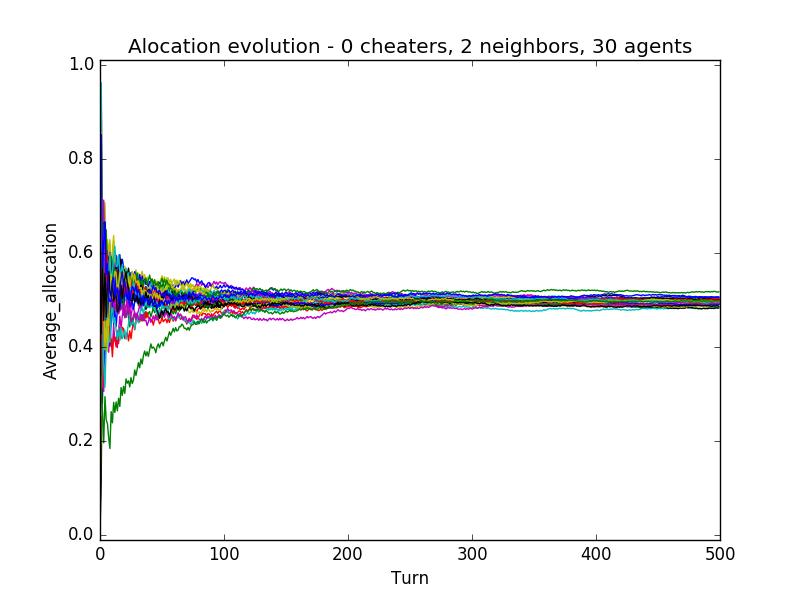
\includegraphics{pics/lpgp_0cheaters_2nei_30agents-alloc.png}
\caption{Allocation in scenario without non-compliant agents. Each
coloured line represents a different agent.}
\end{figure}

\end{frame}

\begin{frame}{Dealing With Non-compliant Behaviour}

\begin{figure}[htbp]
\centering
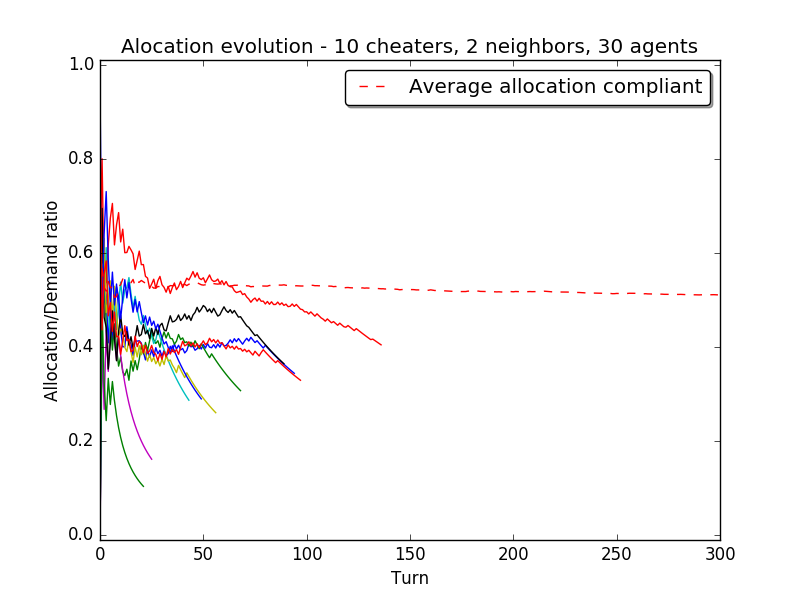
\includegraphics{pics/lpgp_10cheaters_2nei_30agents-alloc.png}
\caption{Individual allocations for non-compliant agents (solid lines)
compared to compliant average (dashed).}
\end{figure}

\end{frame}

\begin{frame}{Exploring Effects of Connectivity}

\begin{figure}[htbp]
\centering
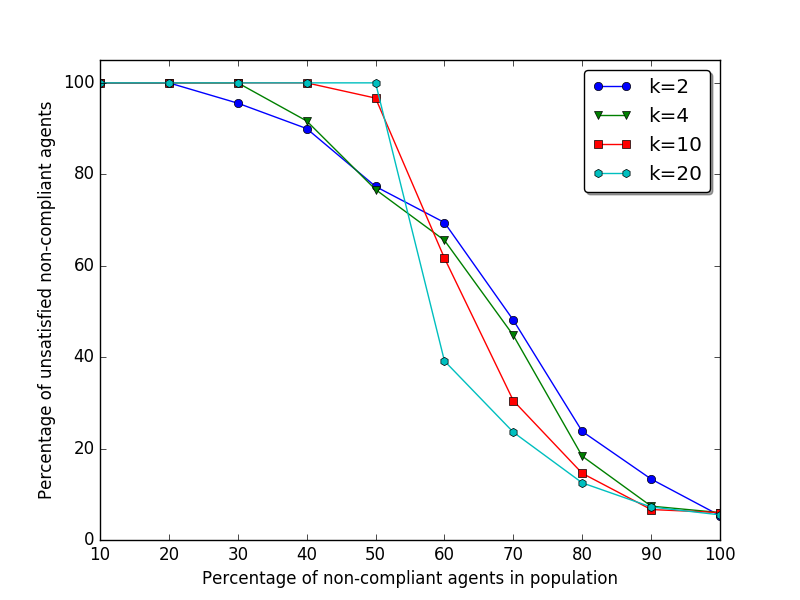
\includegraphics{pics/kgeneral.png}
\caption{Ability of non-compliant behaviour detection, by size of
neighbourhood (\(k\)).}
\end{figure}

\end{frame}

\section{Conclusion}\label{conclusion}

\begin{frame}{Final Remarks}

\begin{itemize}
\item
  Presented solution demonstrate that it is possible to define
  \alert{fair policies of resource allocation} in environments
  characterized by decentralisation, scarcity and no full information
  disclosure.
\item
  Lessons learned:

  \begin{itemize}
  \tightlist
  \item
    Independent subjective assessment of justice can be considered, if
    inserted into a context of \textbf{influence} and \textbf{trust};
  \item
    Authority emerges from \textbf{reputation} autonomously;
  \item
    Ability to aggregate individual, subjective assessments, into
    \textbf{collective, objective facts}.
  \end{itemize}
\item
  Future steps:

  \begin{itemize}
  \tightlist
  \item
    Explore asynchronous game;
  \item
    Distributed pool of resources;
  \item
    Collective mechanisms of verification.
  \end{itemize}
\end{itemize}

\end{frame}

\begin{frame}{Acknowledgemnts}

\begin{itemize}
\item
  National Council for Scientific and Technological Development (CNPq),
  Brazil;
\item
  Diverse colaborators.
\end{itemize}

\begin{figure}
\centering

\includegraphics[width=0.3\textwidth]{cnpq.png}
\end{figure}

\begin{figure}
\centering

\includegraphics[width=0.3\textwidth]{csf.png}
\end{figure}

\end{frame}
